% !Mode:: "TeX:DE:UTF-8:Main"
% arara: pdflatex
% arara: pdflatex
% xarara: convert: {density: 160, otheroptions: -dispose previous -delay 10 -loop 0, format: gif}
%magick -density 160 -delay 15 -loop 0 walkuere.pdf walkuere.gif
\documentclass{beamer}

\usepackage{tikzlings,tikzducks,xfp}
\usetikzlibrary{overlay-beamer-styles}
\setbeamertemplate{navigation symbols}{}
\tikzset{
  hippo1/.pic = {
   \begin{scope}[scale=1.8,transform shape]
     \hippo;
      \begin{scope}[yshift=0.15cm,xshift=-0.5cm,rotate=8]
        \duck[invisible,bowtie]
      \end{scope}
  \end{scope}},
  hippo2/.pic = {
   \begin{scope}[scale=1.6,transform shape]
     \hippo;
  \end{scope}},
  hippo3/.pic = {
   \begin{scope}[scale=1.55,transform shape]
    \hippo
    \begin{scope}[yshift=0.15cm,xshift=-0.5cm,rotate=8]
    \duck[invisible,bowtie]
    \end{scope}
  \end{scope}
  },
  hippo4/.pic = {\begin{scope}[scale=1.7,transform shape]
  \hippo
  \end{scope}
  }
  }
\newcommand\hippoi{0cm}
\newcommand\hippoii{0.5cm}
\newcommand\hippoiii{0.2cm}
\newcommand\hippoiv{0.4cm}

\begin{document}
% https://www.jagderleben.de/sites/default/files/styles/paragraph_2_1_md_2x/public/censhare/22217950/e_Suhle_gut_angenommen.jpg-22217950.jpg?itok=0XbRi79c
% © Matthias Meyer
\begin{frame}<1->[plain,label=hippos]%%%%%%%%%%%%%%%%%%%%%%%%%%%%%%%%%%%%%%%%%%%%%%%%%
\begin{tikzpicture}[remember picture,overlay]
	
% Background image
\node[at=(current page.center)]{%
	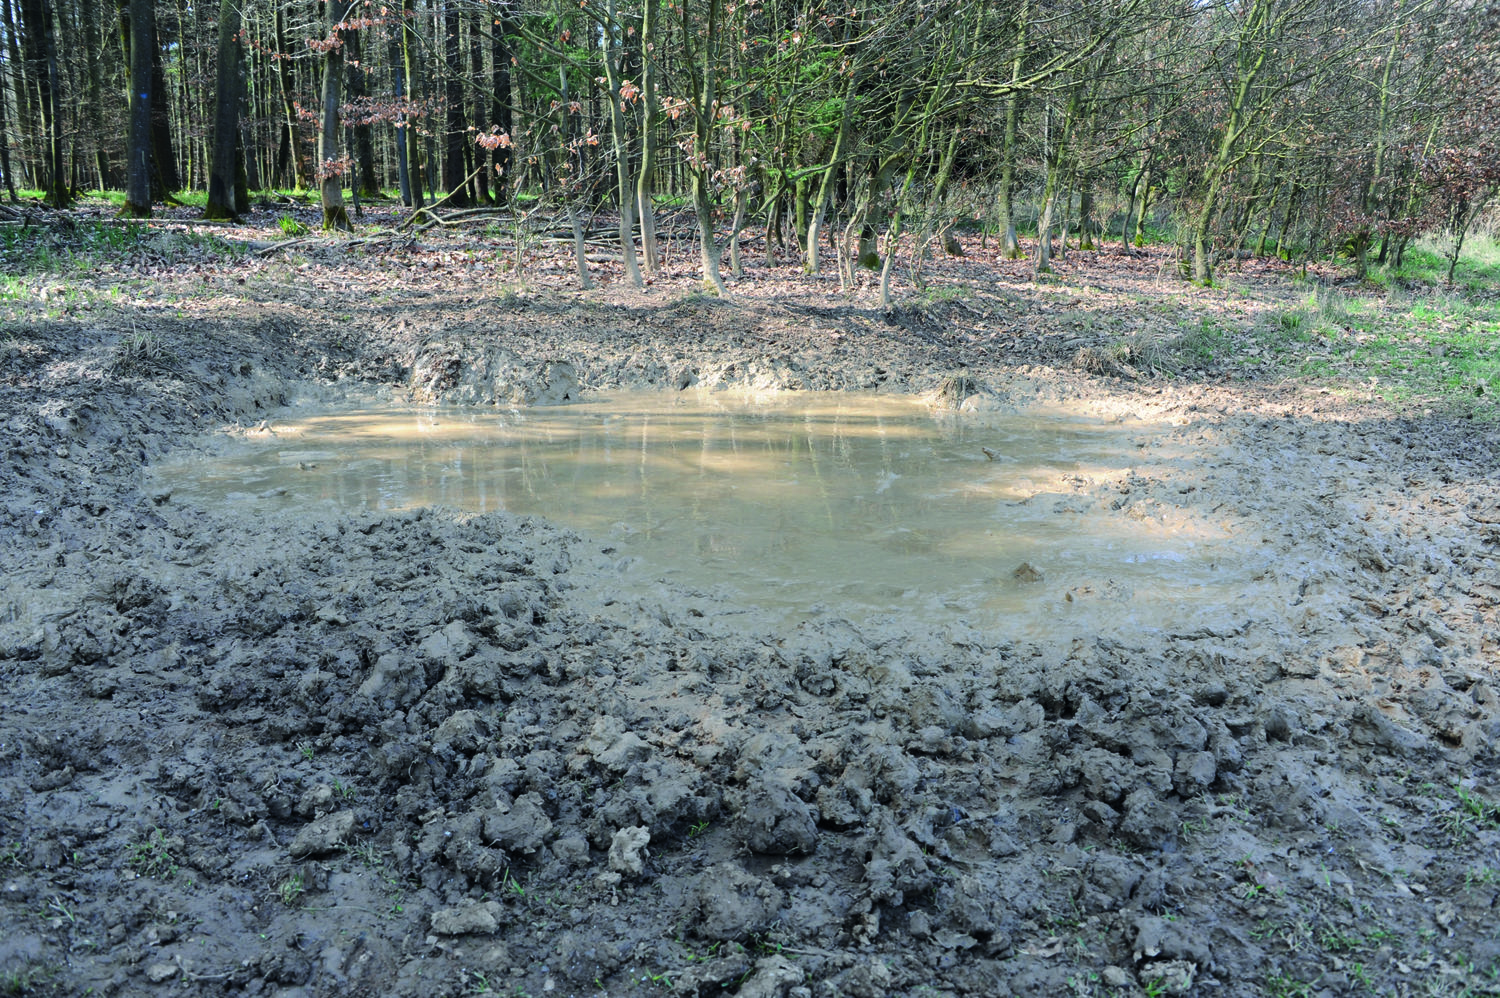
\includegraphics[height=1.05\paperheight]{mud}
};	

% Image credit of background
\node[at=(current page.south east),xshift=-6.6cm,yshift=0.2cm]{%
	\TINY\color{white}© Matthias Meyer
};
\end{tikzpicture}

\vspace*{5cm}\hspace{1cm}

\begin{tikzpicture}[overlay,baseline={(0,0)}]
\path(0,\hippoi) pic {hippo1} -- (3,\hippoii) pic{hippo2} -- (5.5,\hippoiii) pic{hippo3} -- (8.3,\hippoiv) pic{hippo4};
\end{tikzpicture}

\end{frame}
\foreach\i in {0.5,1,1.2,1,0.5}
{
 \edef\hippoi{\fpeval{\hippoi+\i}}
 \setcounter{beamerpauses}{1}
 \againframe{hippos}
}
%\againframe{hippos}
%\againframe{hippos}
%\againframe{hippos}
%\againframe{hippos}
%\againframe{hippos}
%\againframe{hippos}
%\againframe{hippos}
%\againframe{hippos}

\end{document} 